\chapter{Setup}

Hereafter is an image depicting the high level structure of the LORNA project.

\begin{figure}[ht]
    \centering
    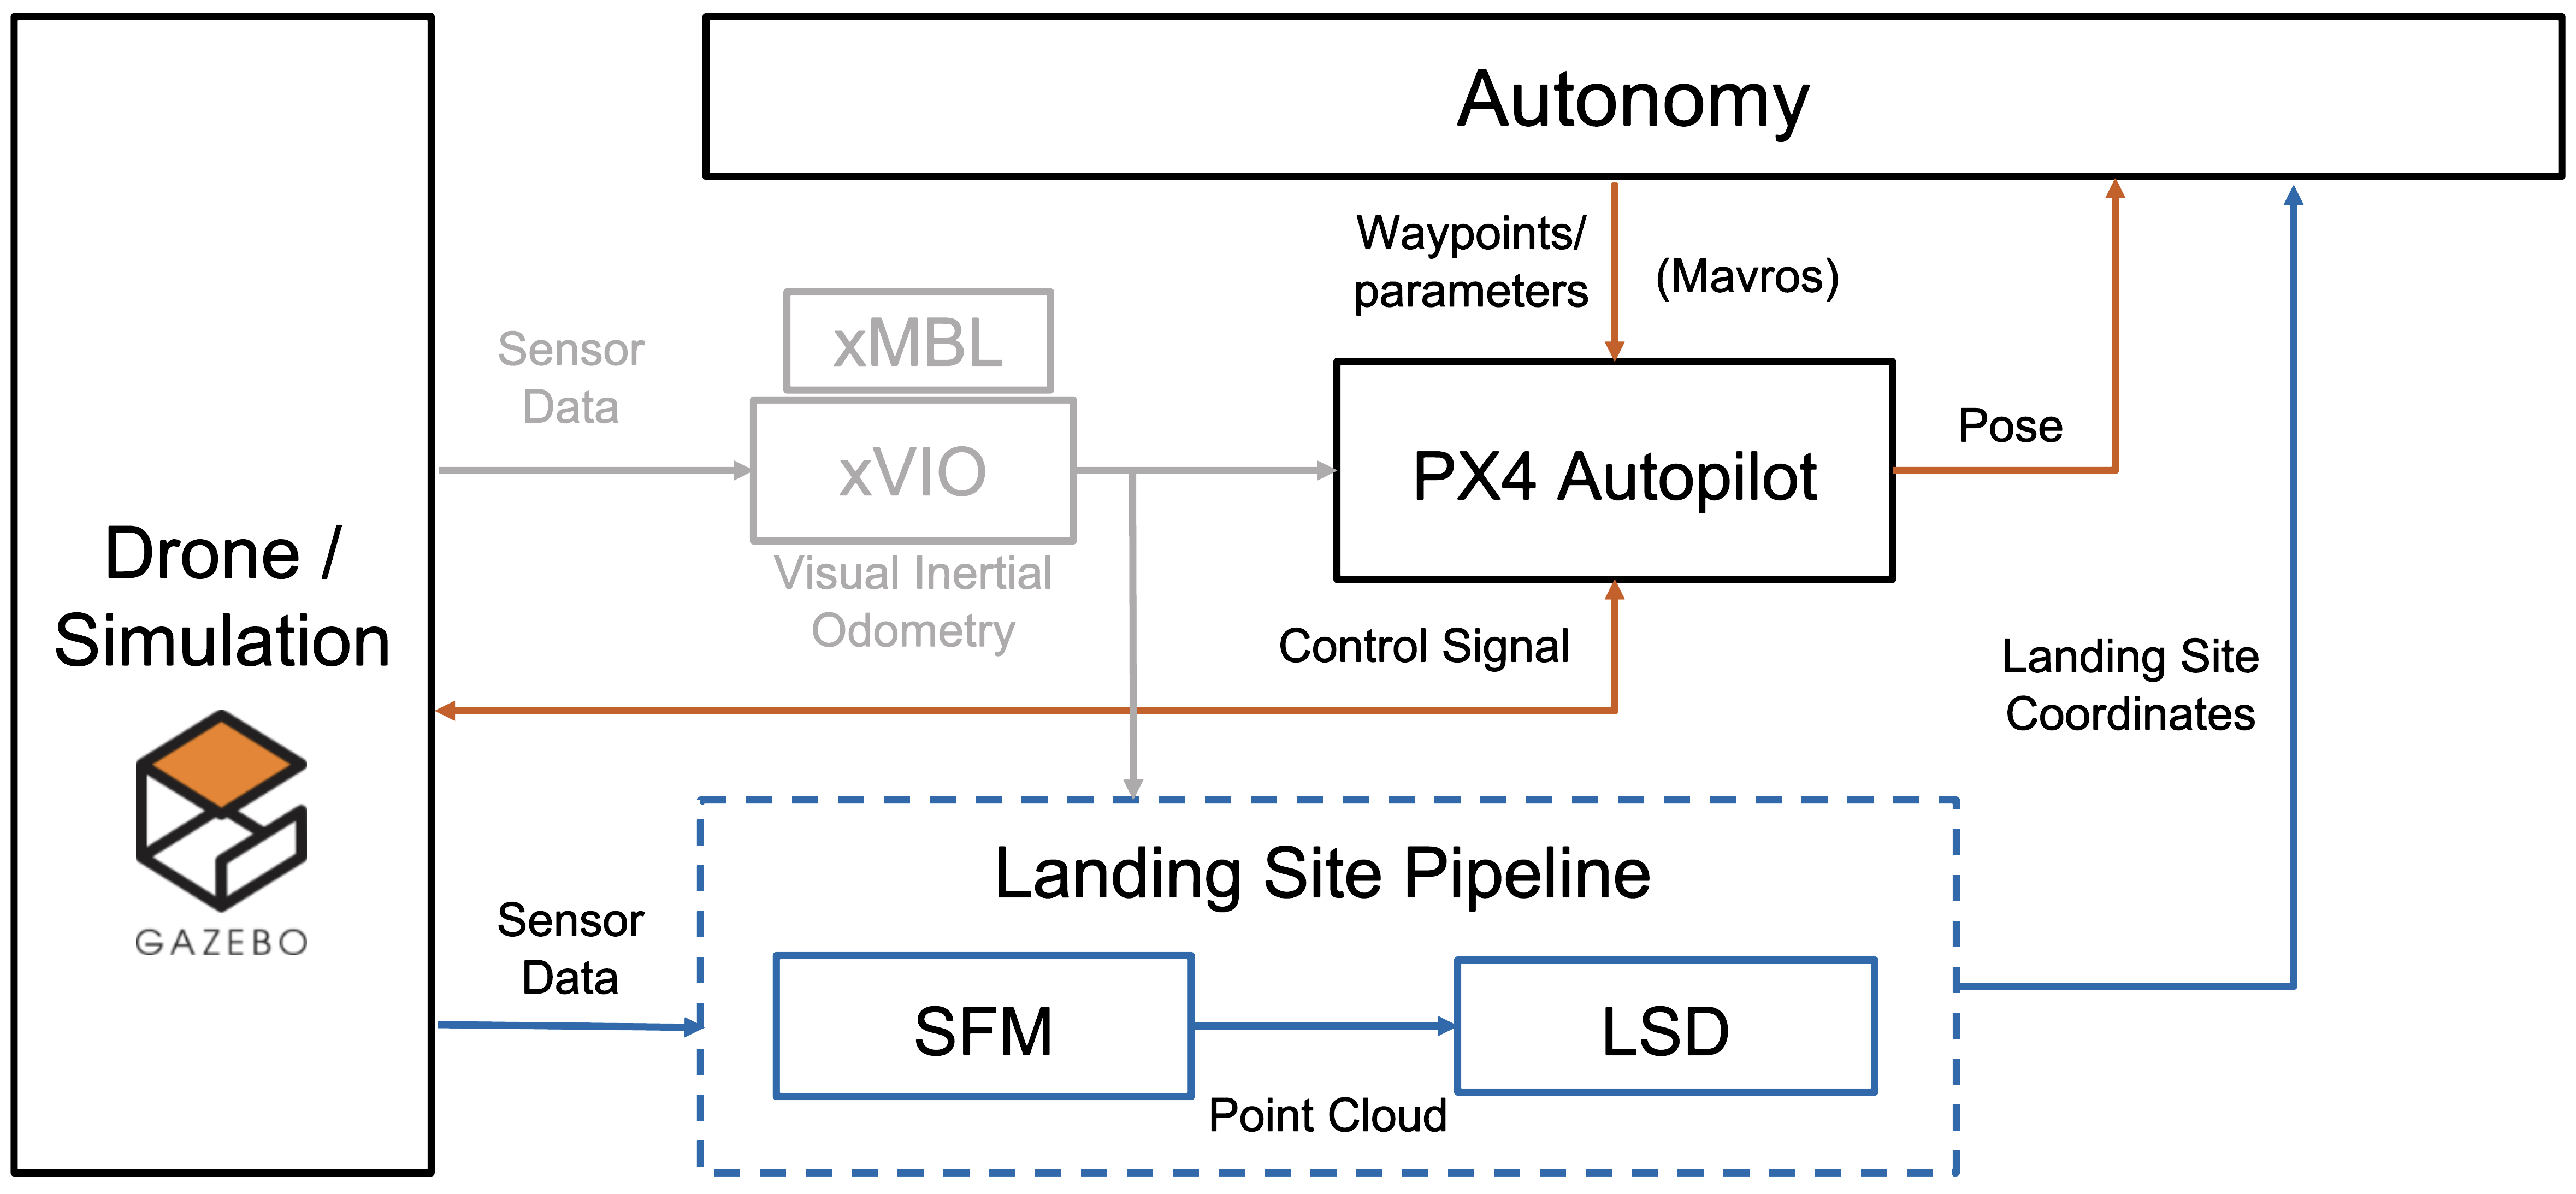
\includegraphics[scale=0.18]{images/setup/setup_flowchart.png}
    \caption{LORNA Project Setup}
    \label{fig:lorna_setup}
\end{figure}

As this thesis revolved around the combination of existing software instances, it is essential to display the individual parts comprising the LORNA project in more detail.

\clearpage %HERE
\section{Simulation}

Despite being able to deploy the landing site detection pipeline onto the voxl2 processor the majority of this thesis was done using a Gazebo Garden simulation of the drone. 

\begin{figure}[ht!]
    \centering
    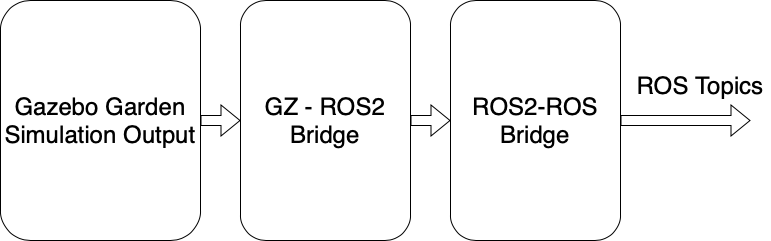
\includegraphics[scale=0.45]{images/setup/GZ_flowchart.png}
    \caption{Gazebo ROS Bridge}
\end{figure}


As the entire software stack of the LORNA project is dependent on ROS instead of ROS2 a bridge was used to convert the sensor information from Gazebo to ROS2 and from ROS2 to ROS.


\section{Landing Site Acquisition Pipeline}\label{sec:setup:LSP}

The landing site acquisition pipeline consists of two nodes. A structure from motion node \citep{SFM} which creates a point cloud using a keyframe based stereo approach on monocular images and a landing site detector node \citep{LSD1, LSD2} which aggregates the depth measurements into a rolling buffer based multi-resolution depth map and segments landing sites on the created DEM. The found landing sites are then supplied to the autonomy. 

\subsection{Structure From Motion (SFM)}\label{subsec:setup:SFM}

\subsubsection{SFM - Bundle Adjustment}

\begin{figure}[ht!]
    \centering
    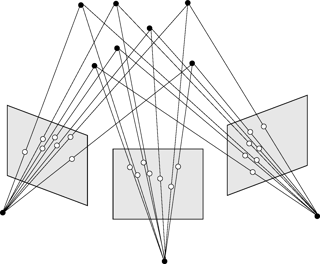
\includegraphics[scale=0.5]{images/setup/BA.png}
    \caption{Bundle Adjustment Procedure}
\end{figure}

In a first step the keyframes are filled with the incoming images and their respective camera pose information. Once the keyframes are filled, each iteration the input as well as all the keyframe poses are refined using a Bundle Adjustment algorithm. 

\subsubsection{SFM - Stereo Depth}

The keyframes and their refined poses are then compared to the new incoming image with regards to image overlap and feature retention. Chosing the most adequate keyframe and the incoming frame, one can create a depth image. The depth image is then converted into a point cloud and packaged together with the respective poses of the images. This allows not only to correctly locate the points in a global frame but also to derive the baseline with which that point cloud was created.

\subsubsection{SFM - Keyframe Updates}

At the end of an iteration the keyframes are updated based on the aforementioned characteristics of image overlap and feature retention quality.

\subsection{Landing Site Detection (LSD)}\label{subsec:setup:LSD}

\subsubsection{LSD - Depth Aggregation}\label{subsubsec:setup:aggregation}

\begin{figure}[ht!]
    \centering
    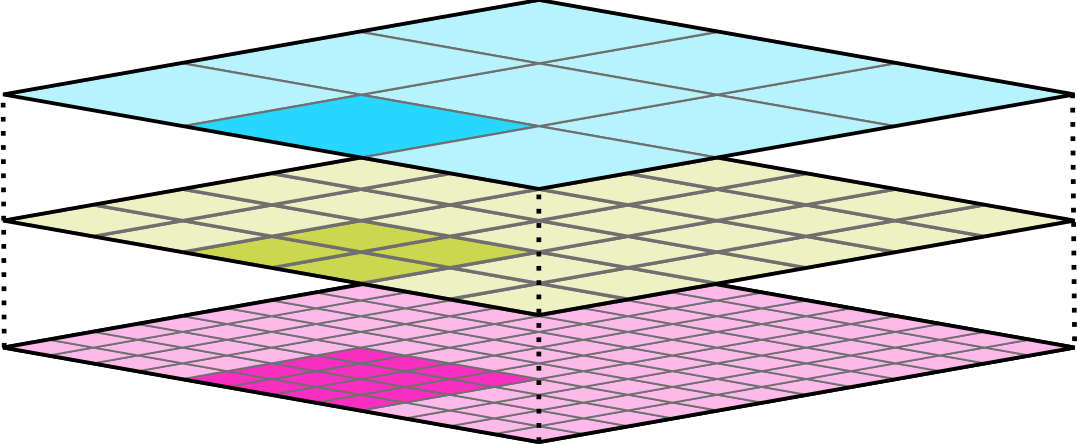
\includegraphics[scale=0.25]{images/setup/DEM.png}
    \caption{Multi Resolution Depth Map}
    \label{fig:DEM}
\end{figure}

The foundation of the landing site detection mechanism is a rolling buffer based multi resolution depth map as indicated in \cref{fig:DEM}. Each base layer cell is represented with 4 cells at a higher resolution layer.

Each point cloud input iteration, the measurements are placed in the respective cells based on the level of detail of the perceived points. In a subsequent step the measurements are pooled up and down the resolution layers in order to make the DEM more consistent and interpolate missing values.

Each cell in this dense elevation map (DEM) is comprised of an optimal mixture of gaussian (OMG) state as described in \citet{LSD2}.

Its update step looks like this:

\begin{align}
    S_t &= S_{t-1} + \sigma_{x_t}^{-2}\\
    \mu_t &=  \frac{1}{S_t}\left(S_{t-1}\mu_{t-1} + \frac{x_t}{\sigma_{x_t}^2}\right)\\
    \sigma_t^2 &=  \frac{1}{S_t}\left( S_{t-1}(\sigma_{t-1}^2 + \mu{t-1}^2) + \frac{x_t^2}{\sigma{x_t}^2} + 1 \right) - \mu_t^2
    \label{eq:OMG_updates}
\end{align}

Where $\mu_t$ is the cell's new mean value, $\sigma_t^2$ is the cell's variance and $S_t$ defines an auxilliary variable to keep track of all past variances within a single scalar.

Thus similar to Kalman filters, the OMG cells' uncertainties decline over time as more measurements are entered. Because of this the DEM's terrain estimate converges over time. 

\subsubsection{LSD - Hazard Segmentation}\label{subsubsec:setup:haz_seg}

On the created depth map landing sites can then be detected. This is done using a roughness and slope assessment of the perceived terrain. Roughness defines the maximum absolute altitude difference around a cell in a certain resolution layer and slope is determined by fitting a plane to the vicinity of a considered point.

If the roughness and slope values lie within the acceptance threshold, the spot is recognized as a landing site and marked as such in a binary landing map. 

\begin{figure}[ht!]
    \centering
    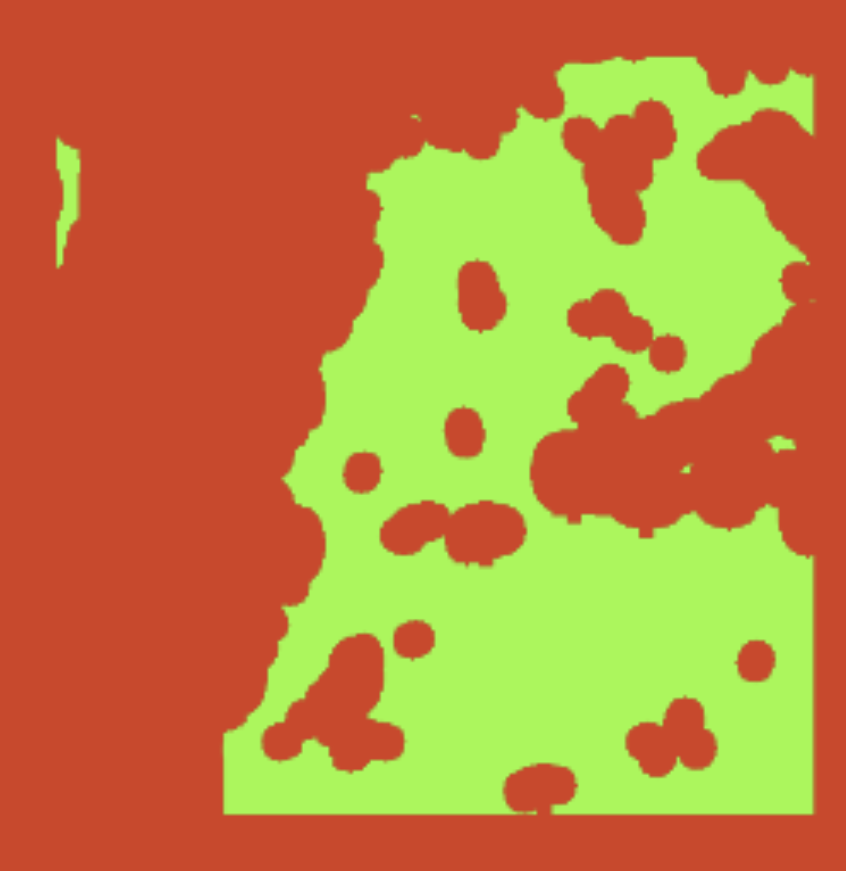
\includegraphics[scale=0.5]{images/setup/ls_map.png}
    \caption{Binary Landing Site Map}
    \label{fig:ls_map}
\end{figure}

\subsubsection{LSD - Landing Site Selection}\label{subsubsec:setup:ls_select}

After applying a distance transform on the landing site map and performing non-maximum suppression on the landing site sizes, the biggest landing sites are found. Their positions are then refined one last time using a mean shift algorithm that considers roughness, uncertainty and size once again. 

\begin{figure}[ht!]
    \centering
    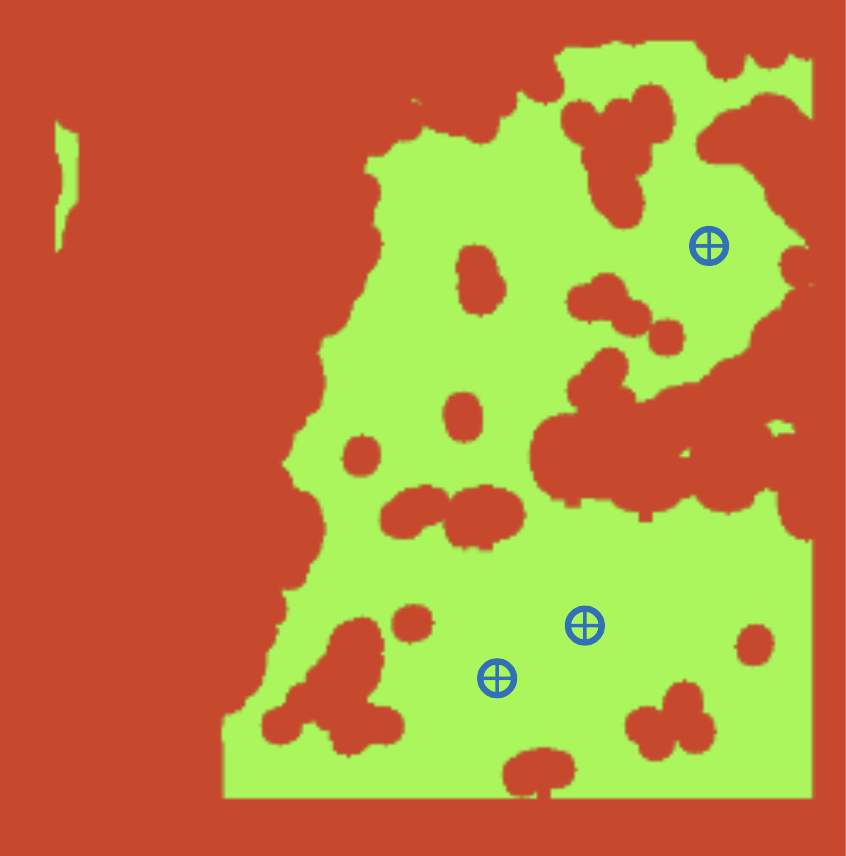
\includegraphics[scale=0.5]{images/setup/ls_map_nms.png}
    \caption{Binary Landing Site Map after Non Maximum Suppression}
    \label{fig:ls_map_nps}
\end{figure}

\clearpage %HERE

\subsubsection{LSD - Debug Images}

\begin{figure}[ht!]
    \centering
    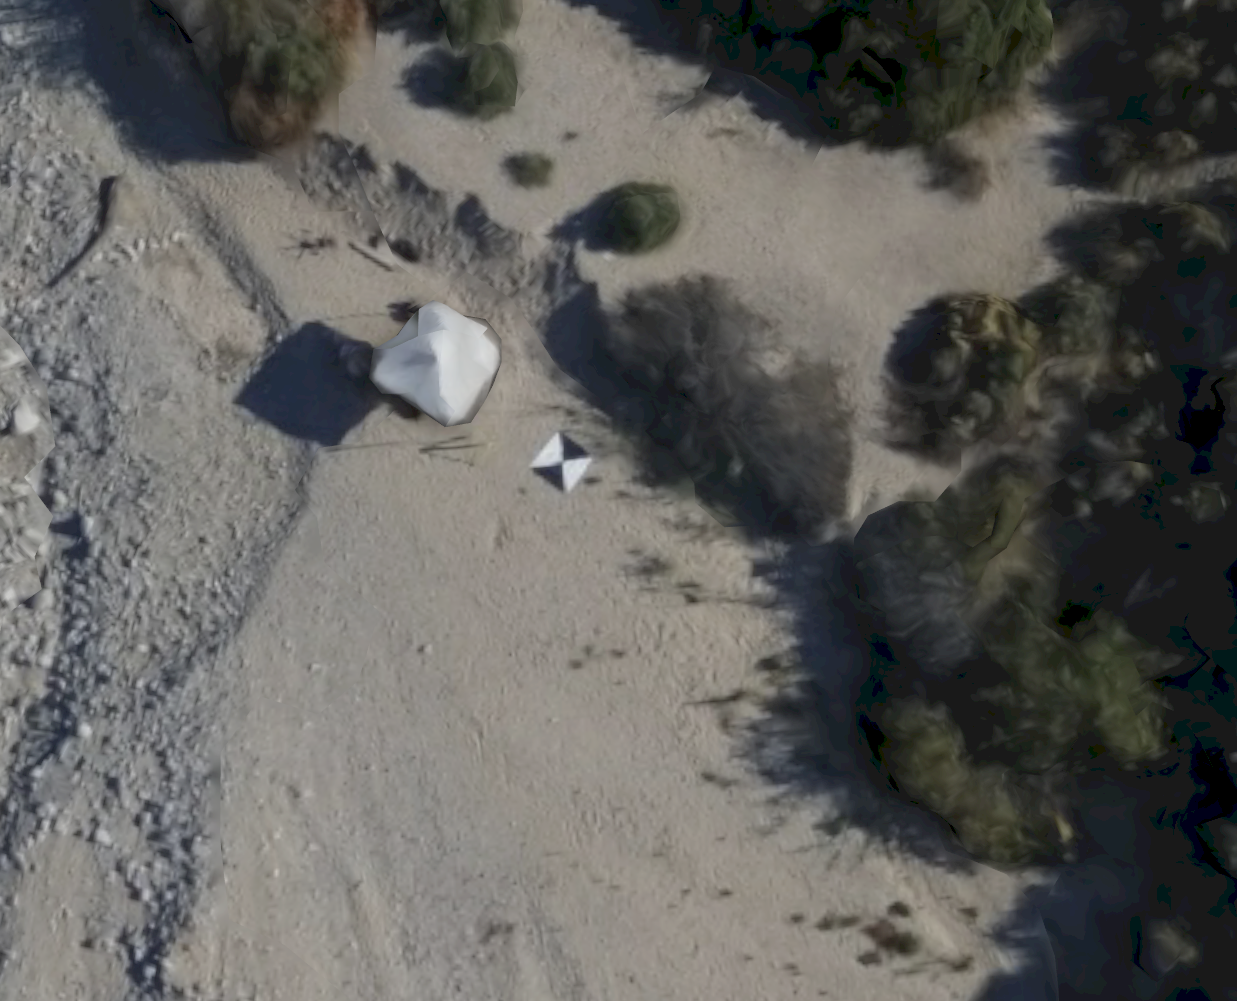
\includegraphics[scale=0.25]{images/setup/lsd_debug_reference.png}
    \caption{Gazebo Simulation Reference}
    \label{fig:lsd_debug_ref}
\end{figure}

\begin{figure}[ht!]
    \centering
    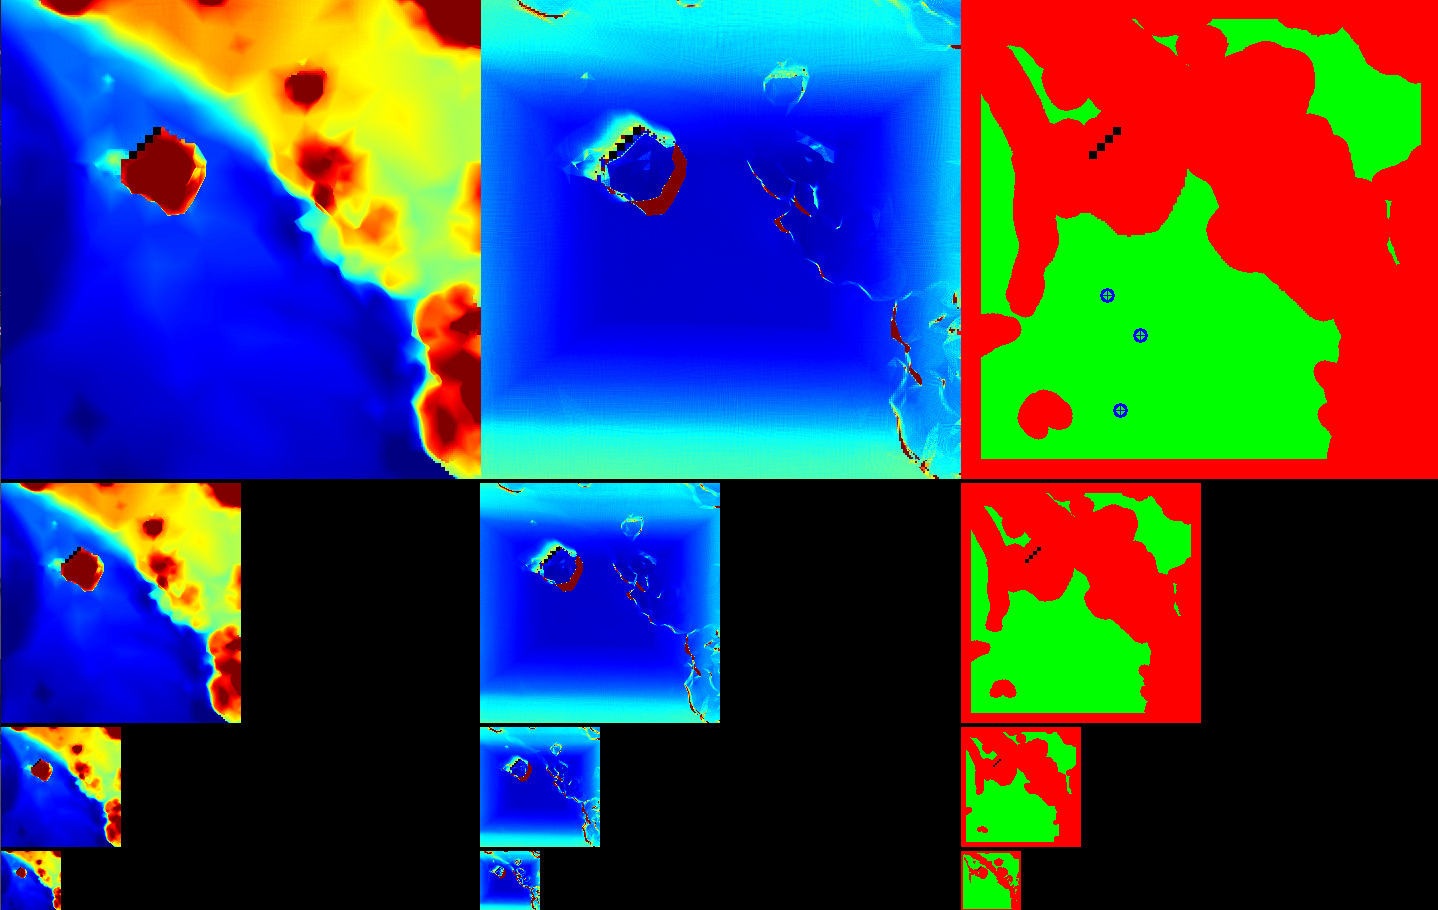
\includegraphics[scale=0.25]{images/setup/lsd_debug_image.png}
    \caption{LSD Debug Image - Left: DEM, Middle: Uncertainties, Right: LS Map}
    \label{fig:lsd_debug}
\end{figure}

The landing site detection debug image is a good comprehensive visualization of the landing spot detection procedure. 

On the left one can see the multi-resolution map displaying the same terrain area in different resolutions. Red pixels are closer, blue further away.

In the middle one can see the uncertainties of the detected points. For simplification purposes the variance of the detected points is simply the associated stereo depth error.

On the right is the above mentioned binary landing site map. Green indicates valid landing sites, and the blue crosses indicate the chosen non-max suppressed and mean shifted landing sites.

\section{Autonomy}\label{sec:setup:autonomy}

The autonomous framework was developed within the LORNA project. It is the overarching instance governing all the necessary behaviors and constituting the interface between all the different nodes of the process. It is connected to the flight controller through the Mavros wrapper of the Mavlink protocol. With this connection it can send waypoints and parameter updates to the flight controller.
In addition to the in \cref{fig:lorna_setup} shown connections it also communicates with a healthguard node keeping track of the systems health state and alerting in case of anomalies.

\begin{figure}[ht!]
    \centering
    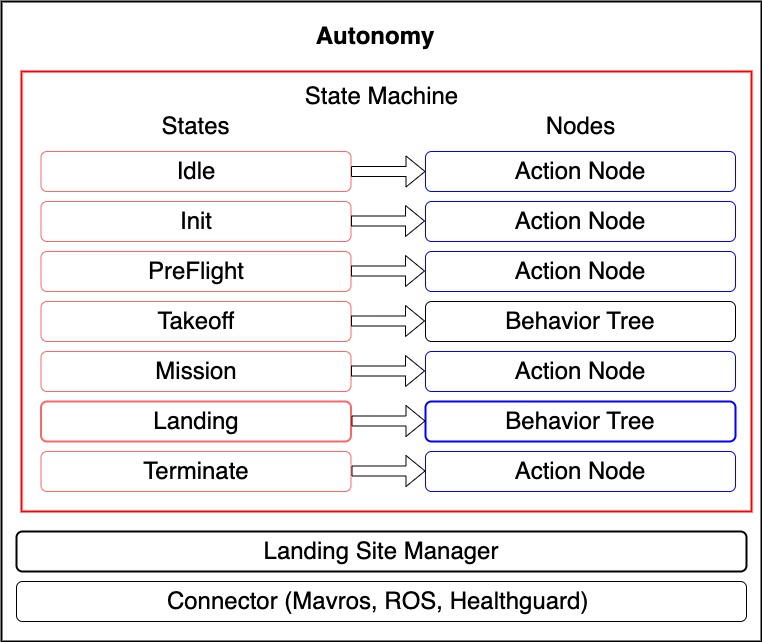
\includegraphics[scale=0.45]{images/setup/autonomy.png}
    \caption{Simplified Structure of the Autonomy}
    \label{fig:autonomy}
\end{figure}

The core of the autonomy is the state machine as depicted in \cref{fig:autonomy}. In each state the respective node is executed which most often is a single action node. For more complicated procedures a behavior tree is used. This is the case for the takeoff as well as the landing node. As indicated in bold, the landing node is the most crucial node in this work as this is where the landing behavior using the landing sites is executed.

In a separate process the landing site manager processes incoming landing sites. Prior to this work the landing site interface was a dummy implementation serving the framework's completeness.

The connector threads interact with the flight controller through Mavros and the other LORNA nodes through a ROS connector.

\subsection{Behavior Tree}

The behavior tree framework within the autonomy is implemented in the traditional way, each comprised of a root node, control flow nodes and action nodes resulting in a modular structure enabling tasks of tremendous complexity. Additionally decorator nodes can be used which alter a single node and function as an add-on on the same level.

\subsubsection{Control Flow Nodes}

The most imported control flow nodes which were used in this thesis are the following:

\begin{itemize}
    \item \textbf{Fallback Node}: Attempts to execute first child node and if successfull returns a success state. Else it continues to the next child node. If no child node was successfull it returns the failure state. A boolean operator analogy for this would be the logical OR, stopping at the first successful entity.
    \item \textbf{Sequence Node}: Executes one child after another. It only returns the success state if all children nodes ran successfully. Otherwise it returns false. Here an analogy would be the logical AND boolean operator.
\end{itemize}

\subsubsection{Decorator Nodes}

The most important decorator nodes are:

\begin{itemize}
    \item \textbf{Inverter Node}: Inverts the output of an action node. Boolean analogon would be the ! (not) operator.
    \item \textbf{Repeat Node}: Repeats a node a number of times until fails or a timeout is reached. 
    \item \textbf{Retry Node}: Similiar to the repeat node loop but it repeats the node a number of times only until it succeeds or a defined timeout is reached.
    \item \textbf{Timeout Node}: Adding a timeout to an action node which otherwise wouldn't be temporally limited.
\end{itemize}

\subsubsection{Action Nodes}\label{subsubsec:setup:action_nodes}

There are a multitude of actions required for the various subtask a rotorcraft has to perform during a mission. The most important ones for the landing behavior in this work are the following:

\begin{itemize}
    \item ChangeAltitudeAction: Changes the drone's altitude to the given value. The ascend / descend velocity diminishes upon reaching proximity to the desired waypoint.
    \item HoldPoseAction: Self-explanatory: the drone holds the current pose for a given time.
    \item LandingAction: Similar to the ChangeAltitudeAction, it descends to a waypoint which in this case is simply the ground vertically below the drone's current position. Upon reaching a certain proximity to the landing point, the descent velocity is reduced to a minimum in order to accomplish smooth landing.
    \item NavigateToWaypointAction: Lateral movement to the given waypoint. Same proximity based slow-down mechanism as ChangeAltitudeAction and LandingAction.
    \item RotateTowardsWaypointAction: Rotates the drone to face the given waypoint.
\end{itemize}








